\chapter{LAYOUT}
%da modificare
La struttura del layout web è stata progettata seguendo questi criteri:
\begin{itemize}
    \item Il \textbf{logo} è stato collocato nell'angolo in alto a sinistra.
    \item Delle \textbf{immagini a scorrimento} sono state inserite per illustrare lo scopo del sito, ossia la vendita di dinosauri e prodotti ad essi correlati.
    \item Un \textbf{menu di navigazione}  posto in alto al centro è stato organizzato per facilitare la selezione di prodotti.
    \item Nel corpo del sito troviamo sulla sinistra i vari \textbf{filtri} per semplificare la ricerca. Accanto possiamo trovare alcuni degli \textbf{articoli} presenti sull'e-commerce. 
    \item Il \textbf{footer} conterrà informazioni di contatto e altre utili risorse.
\end{itemize}
  \begin{figure}[H]
        \centering
        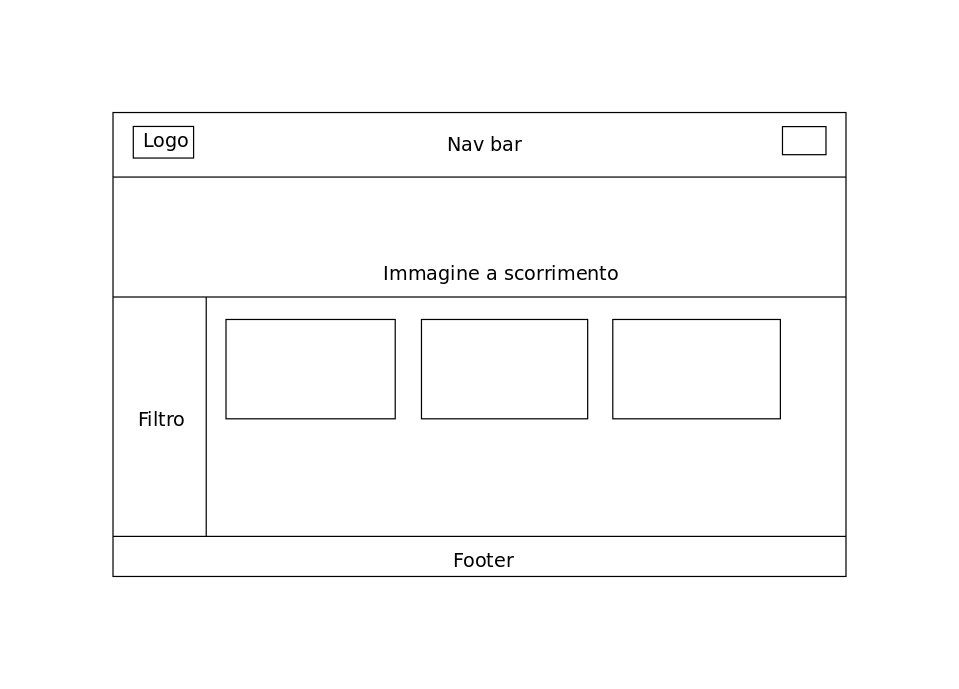
\includegraphics[width=0.80\textwidth]{immagini/desktop_view.png}
        \caption{Visione desktop dell'e-commerce}
    \end{figure}